\documentclass[12pt,oneside]{book}
\include{macros/style}
% Long Table and decimal aligned columns
\usepackage{dcolumn}
\usepackage{longtable}

% Mathematics support
\usepackage{amsmath}
\usepackage{amsthm}
\usepackage{amssymb}


% Text Control
\usepackage{xspace}
\usepackage{textcase}

% Graphics
\usepackage{wasysym}
\usepackage{graphics}
\usepackage{graphicx}   % A package to allow insertion of external image files

\usepackage{svg}
\usepackage{amsmath}


\usepackage{enumitem}% http://ctan.org/pkg/enumitem
\usepackage{subcaption}
\usepackage{xurl}

\usepackage{booktabs,tabularx}
\usepackage{multirow}

\usepackage{algorithm}
\usepackage{algpseudocode}

\newcommand{\GT}[1]{{\color{blue}{\bf [GT: #1]}}}
\newcommand{\TODO}[1]{{\color{red}{\bf [TODO: #1]}}}


\begin{document}

% Front Matter
\input frontmatter/fm

\newpage

	\startfirstchapter{Introduction}
\label{chapter:introduction}

\section{Motivation}

The need for data compression, more specifically entropy coding, was introduced when television transmissions and mobile telephone services started becoming commercial as early as the 1940s \cite{Shannon1948Bell}. Then in the 1950s, with the birth of limited and expensive digital storage devices, researchers (such as David Huffman) have started to develop methods to minimize the redundancy of messages\cite{Huffman1952IRE}. Since then, many data compression schemes have been studied, proposed, and used in all kinds of data including text, audio, and video. With the rapid growth of computing power and the use of different compression schemes, we are now able to send and receive simultaneous real-time high-quality audio and video information in virtual group conferences held on platforms such as Zoom, Google Meet, Skype, etc.

Despite all the mentioned advancements, having cheaper storage devices, and fast internet access, the need for consuming less storage and improving transfer latency is still ongoing. According to Speedtest Global Index, 72 countries out of 182 ($\sim 40\%$) have a slower than 25 Mbps median internet speed over a fixed broadband connection\cite{speedtest}. The 25 Mbps is FCC's recommended connection speed for telecommuting and virtual classrooms\cite{FCC_broadband_2011}. This statistic is even worse for mobile connections, i.e. 68 countries out of 141 ($\sim 48\%$). In addition to the speed, it has been reported that users mostly have a limited amount of download/upload capacity which requires them to pay per their usage. Having said that, especially during the pandemic of COVID-19, it was very difficult for the government and health organizations of these countries to enforce remote working and virtual classes. Hence, all such issues result in the investment of tech companies in the improvement of compression schemes to be able to provide services to more countries and to a wider range of people.

\section{Virtual Music Performance}
\label{sec:virtual-music-performance}

Even though developed countries, with faster and unlimited internet connections, could support remote working and virtual classes during the pandemic of COVID-19, some types of virtual practices are still very difficult or even impossible\cite{bartlette2006effect,chafe2010effect}. One example of such practice is virtual music performances. Unlike a group audio call, in which people can still communicate with one second of latency, having even 100ms latency for a group to perform a music piece together can easily make them out of sync\cite{chafe2004effect,bartlette2006effect}. This is due to the fact that in a group audio call, one person usually waits and listens to another and then speaks when they hear silence. Having one second of latency simply means one second of extra silence between two speakers which is not annoying. In virtual music performance, however, everyone plays simultaneously and the activity of listening and playing happens at the same time. Therefore, the need for reducing the latency of audio is still in high demand and one of the approaches to achieve this reduction is by improving audio compression schemes.

% \TODO{search jack trip}

% \cite{rottondi2016overview}

\section{Domain-Specific Audio Compression} 

One approach to improve audio compression even further is to use a domain-specific scheme. Unlike the \textbf{MPEG Audio Layer III (MP3)} and \textbf{Advanced Audio Coding (AAC)} schemes that are designed to be general-purpose audio compression schemes, a domain-specific audio compression focuses on more restricted use cases. For example, in the virtual music performance scenario, an audio compression scheme which is specifically tailor designed for a single musical instrument can potentially achieve better compression, and consequently, less latency in transmission because the audio signal patterns are more limited and easy to recognize. 

For example, a drum player can produce a limited number of sounds with the drum set that are typically repeated in  predictable patterns. We believe that an audio compression scheme can be specifically designed so that is able to understand and identify all such limited signals and rhythmic patterns and instead of sending repeating signals, should be able to simply refer to the known previously played audio signal. This can become more difficult for a more sophisticated musical instrument like a piano which can play any mixture of 88 different notes with different intensities and duration. In addition, for a musical instrument that can play continuous notes, like a violin or a cello, it would be much more difficult to find patterns.

In this thesis, I will be investigating whether a domain-specific audio compression schema can be designed in order to improve the compression of music with repeating structure without introducing annoying perceptible differences.


\section{Contributions}

The main contributions of the thesis are: 


\begin{itemize}
\item A simplified perceptual audio compression scheme that is based on well-known schemes such as MP3 and AAC but that can be easily implemented and understood in order to explore how audio compression works and experiments variations and modifications without having to deal with the implementation complexities 
of established audio coding algorithms. 

\item A method for leveraging repetition in music to improve audio compression is described, implemented, and tested showing the potential of domain-specific audio compression. 

\item For someone who is interested in evaluating audio compression schemes that leverage music repetition, an experimental methodology is proposed and applied using a 
publicly available dataset. 

\item For programmers who would like to explore the new audio compression scheme closely, the Python source code of the encoder, decoder, experiment, and figures are provided in a public GitHub repository \TODO{Cite} \TODO{say following the reproducibility MIR}.

\item For someone who is interested to follow up on this thesis and investigate approaches for its improvements, some potential ideas for future works are provided in the final chapter.
\end{itemize}

\section{History of the Thesis}

Entering the University of Victoria, following my previous experience and passion for Virtual Reality (VR) and Human-Computer Interaction, I had plans to work around the Music in Virtual Reality as the subject for my thesis. Sadly, with the start of the pandemic of COVID-19, it was very difficult to conduct user studies and potentially expose participants to the virus 
as they would need to use expensive VR equipment that is not widely available. Therefore, I decided to choose my second life-long interest, audio compression, as my thesis without the need to run user studies.

I grew up, experiencing the excitement of compressing my audio and video files to MP3 and MP4. As a curious child, I always wondered how this is possible and if someday, I could do the same. My curiosity grew more when I got older and started working in a video conferencing service provider company. There, I noticed how a carefully chosen audio and video encoder can affect the whole experience of a video conference, and how it plays a major part in a business to be built upon. So I found this opportunity to fulfil my curiosity at the University of Victoria by taking Data Compression courses, taking Directed Studies about Audio Compression Schemes, and working on Audio Compression Schemes leveraging repetition of tones for my thesis.

\section{Thesis Structure}
To help the reader understand the flow and structure of the thesis, the aim and expected contents of each one of the chapters are described below:

\begin{description}
\item[Chapter \ref{chapter:related}] points out some of the published research related to the subject of my thesis in subjects of audio \& video compression, evaluation of audio quality, network music performance, and repetition in sound source separation.
\item[Chapter \ref{chapter:background}] describes some mathematics, techniques, and approaches for the background knowledge and empirical investigations that are required before proposing the new idea in the audio compression.
\item[Chapter \ref{chapter:proposed}] explains the main idea of the new audio compression scheme, then it provides technical considerations and algorithmic implementations, and then it illustrates some results of its execution on a single well-known song.
\item[Chapter \ref{chapter:Exp}] describes an experiment over a diverse music dataset. Results are reported using descriptive and inferential statistical analysis aiming to achieve a more generalizable understanding of the new compression scheme
\item[Chapter \ref{chapter:concl}] provides an overview of the knowledge achieved from chapter \ref{chapter:Exp} and then, by referring to some of the mentioned research in chapter \ref{chapter:related}, some potential improvements are proposed that can be done in the future studies.
\end{description}
	\startchapter{Related Work}
\label{chapter:related}

\newlength{\savedunitlength}
\setlength{\unitlength}{2em}

There is a large amount of related work to the topic of this thesis. In this chapter, an overview of related work is provided grouped 
into particular topics relevant to the thesis and references to the associated literature are provided. 


\section{Lossless Compression}
\label{sec:lossless-compression}

One of the earliest and still widely used forms of entropy coding is \textbf{Huffman Coding}. In a digital storage device, string characters are represented using a fixed number of bits. When a string is converted using Huffman encoding, frequently used characters will be stored with fewer bits and not-so-frequently occurring characters will be stored with more bits, resulting in fewer bits used in total \cite{Huffman1952IRE}. For example, the text "aab" when saved in ASCII code, uses 24 bits. By generating a Huffman Tree, it can be determined to replace the character "a" with the binary "0" and the character "b" with the binary "10". The Huffman coding of the text becomes the binary "0010" which can be stored in 4 bits.

An obvious improvement on Huffman coding is Arithmetic Coding in which instead of replacing each character with a code, the entire message can be encoded into a single number\cite{rissanen1976arithmetic}. Both of these encodings can compress a message significantly, however, they are not suitable for texts with repeated content. For example, Huffman coding of the text "aabaab" is the binary "0010 0010". Similarly, in Arithmetic Coding, the encoded binary of a repeated text consumes almost double the number of bits compared to its singular form.

Therefore, before using the Huffman or Arithmetic Coding, it is typically proposed to reduce the  repetition with \textbf{Run-length encoding (RLE)} in which repeating consequent characters are replaced with the character and the length of its repetition\cite{RLE}. So it changes "aabaab" into "a($\times 2$)ba($\times 2$)b". To reduce the repetition further, it was proposed in LZ77 and LZ78 to look back in the sequence of characters to see if it is a match and reuse it\cite{LZ77, LZ78}. So two numbers are required to mention how many characters to go back and how many of them to use. For example, "aabaab" changes into "a(1,1)b(3,3)". Even though this approach is very promising for lossless compression, the challenging part is implementing a match-finding algorithm as a poor implementation can lead to a lot of process and memory usage in large files. Welch's high-performance implementation of LZ78 (a.k.a LZW) became widely used in UNIX operating system with the \verb|compress| command (\verb|.Z| files) and \verb|.gif| image format\cite{LZW}. Later, by combining the LZ77 and Huffman coding, \textbf{DEFLATE algorithm} was born which is still being used in \verb|.gz|, \verb|.zip|, and \verb|.png| files\cite{Deutsch1996rfc1951}. Some of the more space-efficient, but slower compression schemes are LZMA algorithm, which uses LZ77, Markov Chains, and Arithmetic Coding\cite{igor_pavlov_1998_lzma}, is being used in \verb|.7z|| files and Burrows-Wheeler algorithm, which uses a clever text sorting technique followed by RLE and Huffman coding\cite{burrows1994block}, is being used in \verb|.bz| files.

Even though these algorithms are highly effective on human-readable text files, such as HTML, CSS, and programming source codes, they are far less  effective on raw binary data because they such data is less likely to contain repeating patterns in its raw form. Hence, the algorithms mentioned above are used after different types of lossy transforms and manipulations, described in section \ref{sec:audio-compression} and with even more details in sections \ref{sec:fourier} and \ref{sec:mdct}.

\section{Audio Compression}
\label{sec:audio-compression}

Studies on audio compression began before digital storage devices became widespread. Shannon proposed a logarithmic transformation of the original communication message in the year 1948\cite{Shannon1948Bell}. Later, the Discrete Fourier transform (DFT) was proven to be very useful for audio compaction due to the wave nature of audio signals, more specifically, Discrete Cosine Transformation (DCT) was shown to be very useful in pattern recognition, and scalar-type Wiener filtering\cite{Ahmed1974DCT}. Then, using Time-Domain Aliasing Cancellation (TDAC), a \textbf{Modified version of Discrete Cosine Transform (MDCT)} was designed that is still being used in almost every audio compression scheme today\cite{Princen1986TDAC}. Because of MDCT's importance, it will be described in more detail in section \ref{sec:mdct}.

Since then, many researchers focused on improvements in the MDCT. For example, the MDCT is reported to produce severe artifacts at lower bitrates. To fix this, Sinha and Johnston proposed combining it with wavelet filterbank\cite{sinha_audio_1996}, Dietz et al. developed Spectral Band Replication (SBR)\cite{dietz2002SBR}, Brinker et al. studied Parametric Coding\cite{brinker2002parametric}, and Ravelli et al. proposed using a redundant union of eight MDCT bases\cite{ravelli_union_2008}, which then he showed its benefits in transform-domain audio indexing\cite{ravelli_audio_2010}. 

The first time an audio compression scheme was standardized was in 1993 by the Moving Picture Experts Group (MPEG), consisting of an alliance of groups established by ISO (the International Organization for Standardization) and IEC (the International Electrotechnical Commission). \textbf{The third layer of MPEG-1 (MP3)} standard consists of Polyphase Quadrature Filters (PQF filterbank), MDCT, and cancelling Aliases caused by PQF filterbanks\cite{mpeg1-1993}. The successor of MP3, \textbf{the Advanced Audio Coding (AAC)} standard was introduced in MPEG-2 \cite{mpeg2-1995,bosi1997aac} and then used in MPEG-4 standard in 1999 \cite{mpeg4-2001}. AAC doesn't use the PQF filterbank like MP3. Rather, it uses a pure MDCT followed by Temporal Noise Shaping (TNS) and Perceptual Noise Substitution (PNS). Even though AAC is reported to encode with a better audio quality compared to MP3 in lower bitrates\cite{meares_report_1998}, both of these two widely known standards are able to generate a compressed file with less than 20\% size of the PCM audio signal while the quality difference is guaranteed to be imperceptible.

\begin{figure}[ht]
  \includesvg[inkscapelatex=false,  width=\linewidth]{Figures/chap2/mp3aac.svg}
  \caption{Steps taken for encoding and decoding MP3 and AAC bitstreams.}
  \label{fig:mp3aac}
\end{figure}

Looking at Figure \ref{fig:mp3aac}, we can see that both MP3 and AAC coders receive a PCM audio signal as input, after passing five steps they generate the compressed audio bitstream. The compressed bitstream can be decoded back to the PCM audio signal by passing through inverted versions of those five steps. Three steps are similar in both encoders: MDCT, Scaling \& Quantization, and Huffman Coding. Having said that, I will be focusing more on the first two, specially MDCT, in chapter \ref{chapter:background}. 

Despite being less popular, lossless audio coding has also been receiving attention. Since 2001, the Free Lossless Audio Codec (FLAC) has been an open format developed by Coalson and the Xiph.Org Foundation. Some years later, in 2005, Audio Lossless Coding (ALS) has become standardized in MPEG-4. Unlike MP3 and AAC, both FLAC and MPEG-4 ALS use different types of polynomial or linear models to achieve approximations on small blocks of PCM signal and then they store them alongside their residual difference using the Rice coding\cite{coalson_2001_flac, liebchen_2005_ALC}.

% \TODO{TO include these two? \cite{van2016snare} % \cite{mokry2020audio}}

\section{Evaluation of Audio Quality}

Many lossy audio encoders, including MP3 and AAC, were assessed subjectively to be able to guarantee an "indistinguishable" audio quality \cite{mpeg1-1993,mpeg4-2001}. An experimental design was required for a generalizable result with a limited number of participants who listened to different outputs of these lossy audio codecs and reported their perceived differences among them. One of the most well-known assessment methods that is still being used is called "MUlti Stimulus test with Hidden Reference and Anchor (MUSHRA)" recommended by the International Telecommunication Union (ITU)\cite{MUSHRA}. It involves a series of tests that are recognized to be one of the most reliable ways to measure the quality of audio.

Since subjective quality assessment is expensive and very time-consuming, many studies were made to develop an objective measurement method that is able to achieve an estimate of the perceived audio quality automatically from the signal. Because many of the introduced objective methods such as PESQ\cite{pesq} and PSQM\cite{psqm} were never thoroughly validated, ITU studied six methods and integrated their promising tools into one single method called \textbf{Perceptual Evaluation of Audio Quality (PEAQ)} \cite{peaq}. PEAQ was carefully validated and it was proven to generate reliable and useful information for some applications. There have been some doubts that PEAQ represents a realistic and valid model of auditory perception because it is a composite of multiple different auditory models, several secondary feature extraction techniques and an artificial neural network. Therefore, even though the PEMO-Q method was proposed which simplifies and slightly improves the PEAQ\cite{huber2006pemo}, PEAQ is still considered to be useful enough to predict subjective audio quality ratings.

PEAQ was examined and implemented by Kabal and other graduate students at McGill University as part of a course project\cite{kabal2002examination} and their implementation was used for this thesis. In chapter \ref{chapter:background}, I will be describing this method and its implementation in more detail.

\section{Repetition in Sound Source Separation}

After efficient algorithms were proposed for \textbf{Non-negative Matrix Factorization (NMF)}\cite{nmf} and showed its ability to identify components with temporal structure\cite{smaragdis2004non}, attempts were made to use it to separate audio objects (such as tones)\cite{smaragdis2004discovering} and even vocal tracks\cite{vembu2005separation} in an audio signal. Because this approach was dependent on particular initialization, features, and prior training for each type of audio, Rafii and Pardo proposed a new method that is based on "self-similarity" and works on any audio as long as it has a repeating structure (such as a piece of music). 

At first, they named their method \textbf{REpeating Pattern Extraction Technique (REPET)} and proposed to segment the audio at the found period of the repeating structure. Then, by averaging segments, they create a repeating segment model which is compared to the original audio to label it as the foreground audio (vocal) or the background (instrumental companions)\cite{rafii2011simple}. Later, Rafii and Pardo improved their method using a similarity matrix\cite{rafii_musicvoice_2012}, noise estimation with an "online" sliding buffer(REPET-SIM)\cite{rafii2013online}, and by taking the element-wise median of all the periodically repeating segments\cite{Rafii2013repet}. Later, supervised by Pardo, Seetharaman proposed to use a 2D Fourier Transform of the audio spectrogram\cite{seetharaman_musicvoice_2017}.

There are many different REPET implementations on the internet, one of which is in the nussl python package implemented by Manilow, Seetharaman, and Pardo\cite{nussl} which I used for this thesis. In chapter \ref{chapter:background}, I will be describing this algorithm in more detail.

% \cite{spleeter2020}

\section{Network Music Performance}

As already mentioned in section \ref{sec:virtual-music-performance}, having even 100 milliseconds of delay between two music performers can easily make them out of sync \cite{chafe2004effect,bartlette2006effect}. In a Network Music Performance (NMP), the time delay is split into 12 different steps starting from the music instrument, transmitting to the network, and to the ear of the other person. These steps are known as Over-all One-way Source-to-Ear (OOSE) and each step contributes differently to the amount of delay between two performers\cite{carot2009fundamentals, rottondi2016overview}.

It is reported that choosing between different audio encoders can significantly affect the OOSE delay. Lutzky has reported a comparison of the algorithmic delay between MP3 and AAC audio encoders which shows at least 20 ms of delay\cite{lutzky2004guideline}. This is hardly acceptable for the OOSE delay budget. Therefore, attempts were made to develop low-delay audio encoders such as ultra-low-delay (ULD)\cite{schuller2002perceptual}, CELT\cite{valin2009full}, and OPUS\cite{valin2016high} encoders which were able to achieve delays as low as 4 ms. 


% However, \TODO{why aren't they useful?}

\section{Similarity-based Audio Compression}

There has been limited work directly 
related to leveraging repetition for audio compression which is the main idea of the thesis. A related approach has been termed similarity-based audio compression. Cunningham et al. developed an audio compression scheme named ACER (Audio Compression Exploiting Repetition) by finding repeating matches in the audio\cite{cunningham2005play}, and then they tried different approaches for its improvement such as: by using static and dynamic block searches\cite{cunningham2007advances} and a similarity matrix \cite{cunningham2014data}. They developed a file format\cite{cunningham2009audio} and evaluated it objectively and subjectively\cite{cunningham2013initial,cunningham2019subjective}. The achievements of Cunningham et al. show promising results in the improvement of audio compression. However, they believed more improvements are needed in the search for matching signals as their approaches were mostly not efficient. Recently, Tarjano and Pereira proposed an efficient approach to segment "quasi-periodic" audio signals and despite not seeing improvements in the compression rate, they believe this can be beneficial in lossy audio compression applications\cite{tarjano2022efficient}.
	\startchapter{Background and Empirical Investigations}
\label{chapter:background}

In this chapter, I will be describing topics that are 
important for understanding the main ideas behind this thesis. This background material was crucial for me 
to learn well and it was acquired through courses, 
directed studies, and empirical investigations. In each section, the necessary background in terms of mathematics, techniques, and approaches is presented targeting a reader 
who is not necessarily familiar with audio compression. 


\section{Fourier Transformation (FT)}
\label{sec:fourier}

The Fourier Transform is fundamental in audio signal processing. Raw audio signals consist of waves similar to figure \ref{fig:idct} that are difficult (sometimes impossible) to interpret and process without transforming into the frequency domain. The Fourier Transform is one of the most well-known initial steps for processing audio signals. A \textbf{Fourier Transform (FT)} decomposes functions depending on time into functions depending on frequency. It is based on the Fourier Series expansion shown in equation \ref{eq1:fourier-series}, It uses an integral (or "continuous sum") that exploits properties of sine and cosine (with period $P$) to recover the amplitude ($A$) and phase ($\varphi$) of each sinusoid in a Fourier series (Equation \ref{eq1:fourier-series}). The inverse Fourier transform recombines these waves using a similar integral to reproduce the original function.

\begin{equation}
\label{eq1:fourier-series}
s_{\scriptscriptstyle N}(t)={\frac {A_{0}}{2}}+\sum _{n=1}^{N}A_{n}\cdot \cos \left({\tfrac {2\pi }{P}}nt-\varphi _{n}\right)
\end{equation}

In digital signal processing, the \textbf{Discrete Fourier Transform (DFT)} converts a finite sequence of equally-spaced samples of a function into a same-length sequence of equally-spaced samples of the \textbf{Discrete-Time Fourier Transform (DTFT)}, which is a complex-valued function of frequency. Focusing on real values only, the \textbf{Discrete Cosine Transform (DCT)} is a widely used transformation technique in signal processing and data compression \cite{Ahmed1974DCT}. For example, figure \ref{fig:idct} shows a sum of cosine waves at 10, 20, 30, 40, and 50 Hz (equation \ref{eq1:sum-five-freq}) which is difficult to process and store. Figure \ref{fig:dct} is the DCT of the same function which clearly shows its compression potential by having many zeroes.

\begin{equation} 
\label{eq1:sum-five-freq}
A(t)=\sum_{n=1}^{5}n\cos(nwt),\quad w=10\times2\pi
\end{equation}

\begin{figure}[ht]
\centering
\begin{subfigure}{0.45\textwidth}
    \includesvg[width=\linewidth]{Figures/chap3/dct/idct.svg}
    \caption{Raw Audio Signal}
    \label{fig:idct}
\end{subfigure}
\hfill
\begin{subfigure}{0.45\textwidth}
    \includesvg[width=\linewidth]{Figures/chap3/dct/dct.svg}
    \caption{Discrete Cosine Transform}
    \label{fig:dct}
\end{subfigure}
\caption{Sum of cosine waves at 10, 20, 30, 40, and 50 Hz}
\label{fig:dct-idct}
\end{figure}

Fourier transforms can also treat non-periodic functions as periodic with an infinite period. This can generate approximate frequency domain representations of non-periodic functions, allowing a waveform to be converted between its time-domain representation and its frequency domain representation. One realistic example can be seen in figure \ref{fig:piano-wav-spec} which shows a recording of an acoustic piano which plays DEFGAGFEF notes in a raw waveform (\ref{fig:piano-wav}) and a heat map of the time-frequency domain, a.k.a Audio Spectrogram (\ref{fig:piano-spec}).

\begin{figure}[ht]
\centering
\begin{subfigure}{0.49\textwidth}
    \includesvg[width=\linewidth]{Figures/chap3/dct/PianoWav.svg}
    \caption{Raw Audio Recording}
    \label{fig:piano-wav}
\end{subfigure}
\hfill
\begin{subfigure}{0.49\textwidth}
    \includesvg[width=\linewidth]{Figures/chap3/dct/PianoSpec.svg}
    \caption{Audio Spectrogram}
    \label{fig:piano-spec}
\end{subfigure}
\caption{A recording of an acoustic piano playing DEFGAGFEF notes}
\label{fig:piano-wav-spec}
\end{figure}

\section{Non-Negative Matrix Factorisation}
\label{sec:nmf}

During our initial investigations on instrument-specific audio compression schemes we explore sound source 
separation and transcription approaches based on Non-Negative Matrix Factorisation (NMF). NMF factorizes a matrix $V$ into two matrices $W$ and $H$ without any negative elements. When used in MIR, these matrices are spectrograms or some other form of time-frequency representation. 

The relationship between these three matrices is shown in the equation \ref{eq1:nmf}. One of the applications of NMF in digital audio processing is that when the output of FT of audio containing repeating tones, as a matrix consisting of frequencies as rows and time as columns ($V_{f\times t}$), is provided to this algorithm with the right number of extraction tones ($n$), it will generate a matrix containing the frequencies of each tone ($W_{f\times n}$) and a matrix containing the activation time of each tone ($H_{n\times t}$). Multiplying the tones and activation matrices will recreate a matrix similar to $V$. Saving the $W$ and $H$ matrices will consume less space as compared to saving the $V$ and it has the potential to be used as a compression scheme.

\begin{equation} 
\label{eq1:nmf}
f\big(V_{f\times t}\quad,\quad n\big)\quad=\quad W_{f\times n} H_{n\times t} \quad\simeq\quad V_{f\times t}
\end{equation}

So to try the scheme, using LibRosa in Python\cite{mcfee2015librosa}, I provided 12 seconds of acoustic piano sound (similar to figure \ref{fig:piano-spec}) to DFT to obtain a spectrogram matrix $V_{2048\times 572}$. Then NMF was applied using the {\it decompose} function from the {\it librosa} library with $n=15$ 
to generate two matrices of dimensions $W_{2048\times 15}$ and $H_{15\times 572}$. This means the total number of elements to save after the factorization would be 39,300 as compared to 1,171,456 elements after the DFT ($Ratio=3.35\%$). This would be a significant improvement in compression ratio compared to MP3 ($Ratio=15.9\%$). However, listening to the reconstructed $V$ was very annoying ($ODG=-3.793$). Using $n=150$, listening to the reconstructed $V$ was still very annoying ($Ratio=33.5\%, ODG=-3.793$). This means that to factorize two matrices of tones and activations, many important pieces of audio are removed due to careless approximations of the NMF approach.
The {\bf Objective Difference Grade} ODG is a way to 
automatically computed the perceived quality of an audio signal and is explained in the section \ref{sec:peaq}. 
Although the initial investigation of using an NMF-based approach for audio compression was not successful, it provided insights that led to the development of the proposed algorithm. 

\section{Perceptual Evaluation of Audio Quality}
\label{sec:peaq}

Perceptual Evaluation of Audio Quality (PEAQ) \cite{peaq} is a standardized approach used for objective measurements of perceived audio quality, and is based on generally accepted psycho acoustic principles. The overall goal of this algorithm is to obtain a quality comparison measure between two audio files, one as a reference and one decoded from the compressed version of the audio, similar to a \textbf{Subjective Difference Grade (SDG)} acquired from listening tests with human participants. This output is called the \textbf{Objective Difference Grade (ODG)}. The ODG ranges from $0$ to $-4$ and is defined as follows:

\begin{enumerate}[noitemsep]
    \item [0] = Imperceptible
    \item [-1] = Perceptible, but not annoying
    \item [-2] = Slightly annoying
    \item [-3] = Annoying
    \item [-4] = Very annoying
\end{enumerate}

% Sadly, a complete implementation of PEAQ couldn't be found on the internet, so Kabal's Matlab implementation of the algorithm is used outside of this notebook and results are provided for you.

Unfortunately, a complete implementation of PEAQ in Python could not be found. Instead, we utilized Kabal's original MATLAB implementation of the algorithm \cite{kabal2002examination} and loaded the results of the evaluation to integrate with the Python code.

When running the PEAQ algorithm, one important thing to remember is that the audio shouldn't be shifted. Some audio codecs, specifically AAC, apply some paddings in their calculations. For our case, I noticed that there is 1024 sample padding in the decoded signal from the AAC codec. So I had to shift the signal back to be able to get the true ODG result.

\section{Repeating Pattern Extraction Technique}
\label{sec:repet}

As already mentioned in section \ref{sec:lossless-compression}, most general-purpose lossless compression schemes such as DEFLATE\cite{Deutsch1996rfc1951} are not able to compress unmodified variations of DFT or DCT because they are not able to find any repeating patterns. Another idea that was investigated early during my research was to use the DEFLATE algorithm after the audio is split using \textbf{REpeating Pattern Extraction Technique (REPET)}\cite{Rafii2013repet}. REPET is able to create two masks separating the foreground and background audio ($M_{fg} ,  M_{bg}$) based on identifying  repeating patterns. Rafii and Pardo believe that background audio consists of many repeating tones related to instruments, drums, and bases while foreground audio doesn't have repetitions and is mostly related to vocal sounds. Therefore, REPET can be used to remove the sound of the singer and generate suitable karaoke pieces of music. More importantly, as shown in equation \ref{eq1:repet} foreground audio ($A_{fg}$) and background audio ($A_{bg}$) can regenerate the original audio ($A_{orig}$) using a simple add operation. I will refer to this regenerated audio as \textbf{the sum} of REPET's foreground and background.

\begin{equation}
\label{eq1:repet}
\begin{aligned} 
A_{fg} &= A_{orig} \times M_{fg} \\
A_{bg} &= A_{orig} \times M_{bg} \\
A_{fg} + A_{bg} &= A_{orig}
\end{aligned}
\end{equation}

I hypothesized that the DEFLATE algorithm should be able to compress REPET's foreground more than the sum on songs that contain fewer vocals as compared to instrumental music. Moreover, I hypothesized that the DEFLATE algorithm should be able to compress REPET's background more than the sum because they contain more obvious repeating patterns. Later in chapter \ref{chapter:Exp}, these two hypotheses are being tested with an experimental study.

\section{Modified Discrete Cosine Transform}
\label{sec:mdct}

The modified version of Discrete Cosine Transform (MDCT), as already mentioned in section \ref{fig:mp3aac}, is a common step in both MP3 and AAC compression schemas. One important reason for not using DCT in audio compression schemes is that, after the inverse transformation, a quantization error appears in the time domain (figure \ref{fig:piano-dct}). Therefore, the MDCT was developed to have time-domain aliasing cancellation (TDAC) using an overlapping pre-filter technique\cite{Princen1986TDAC}. In a lapped transformation, as shown in figure \ref{fig:lapped-dct}, subsequent wave blocks are overlapped so that the last half of one block coincides with the first half of the next block. When lapping is paired with DCT, it prevents energy leakage into its higher-frequency bins (figure \ref{fig:piano-mdct}), and as a result, more energy is compacted into the DC component. As a result of these advantages, the MDCT is the most widely used time-frequency transformation used in lossy compression techniques in audio data compression.

\begin{figure}[ht]
  \includesvg[width=\linewidth]{Figures/chap3/mdct/lapped.svg}
  \caption{A lapped transform, consisting of the DCT with pre-filters ($P$) and post-filters ($P^{-1}$) straddling block boundaries\cite{christopher_montgomery_next_2013}}.
  \label{fig:lapped-dct}
\end{figure}

Figure \ref{fig:piano-dct-mdct} shows the advantage of MDCT over DCT for audios signals clearly. In \ref{fig:piano-dct} specifically, quantization errors are visible as vertical lines that repeat throughout the time domain. In \ref{fig:piano-mdct} however, not only the time-domain aliasing is cancelled, but it can also be seen that energies in frequency bins are more concentrated in lower frequencies, making the figure darker as compared to the Spectrum and DCT. As a result of all these benefits, the MDCT is very suitable for audio data compression.

\begin{figure}[ht]
\centering
\begin{subfigure}{0.32\textwidth}
    \includesvg[width=\linewidth]{Figures/chap3/mdct/piano-full-spec.svg}
    \caption{Spectrum}
    \label{fig:piano-full-spec}
\end{subfigure}
\hfill
\begin{subfigure}{0.32\textwidth}
    \includesvg[width=\linewidth]{Figures/chap3/mdct/piano-dct.svg}
    \caption{DCT}
    \label{fig:piano-dct}
\end{subfigure}
\hfill
\begin{subfigure}{0.32\textwidth}
    \includesvg[width=\linewidth]{Figures/chap3/mdct/piano-mdct.svg}
    \caption{MDCT}
    \label{fig:piano-mdct}
\end{subfigure}
\caption{DCT and MDCT applied on a recording of an acoustic piano playing DEFGAGFEF notes}
\label{fig:piano-dct-mdct}
\end{figure}

\section{A Simple Lossy Audio Compression Scheme}
\label{sec:simple}

In order to better understand the building blocks of perceptual lossy audio compression, a simple stream-lined lossy audio compression scheme 
was designed and implemented. This allowed more easy experimentation without having to deal with all the implementation complexities of a fully developed audio coder while still retaining the main characteristics of such audio coders. 

Once the MDCT is applied to an audio signal, the resulting data is typically encoded using some form of entropy-based encoding in order to compress it while still retaining the critical and perceptual parts of the signal. In section \ref{sec:audio-compression}, many different approaches for such encoding were introduced. These techniques are carefully designed and modified to find correct parameters that would keep the compressed difference imperceptible. Unfortunately, I didn't have enough time to go through each one of the steps individually to be able to implement a full-blown MP3 or AAC encoder. Instead, I decided to implement  multiple simple proof-of-concepts steps and report the Compression Size Ratio and Audio Quality of each step. For checking the Audio Quality, unlike MP3 and AAC that recruited humans for scoring, I used the ODG in the PEAQ method (described in section \ref{sec:peaq}). My aim during such streamlined steps was to modify frequency bins so that when $M$ is given to a standard DEFLATE algorithm, I could achieve a better compression ratio. It reasonable to assume that any observed differences in compression ratios in the streamlined scheme would most likely result in similar improvements. 

The outcome of each step is shown in Table \ref{tab:piano-lossy-steps} and the decoded wave audio of each step can be found in the Github repository of the project\cite{github2022thesis}.

\begin{description}
    \item[Step 1:] Thanks to Nils Werner's MDCT Python package\cite{werner2020mdct}, I had no problem getting the coefficients matrix ($M$). The MDCT function receives raw wave audio signals ($W$) and returns the matrix of coefficients with 512 frequency bins per frame in the time domain ($t$). It is important to mention that in Python, each element of $W$ is 16-bits and the element size of $M$ is 64-bits. Even though it is nice to have high precision, storing the matrix would require a lot more space compared to $W$. Therefore, I changed the data type of $M$ back to 16-bit numbers. As a result of this step, I achieved only 91\% of the original size while changes in the decoded sound quality were imperceptible.
    
    \item[Step 2] One of the most simple techniques that can improve the compression ratio, is to zero out all high frequencies. It was mentioned earlier that human ears can not perceive extreme high frequencies. This frequency limit is different for each individual, and different lossy audio compression schemes have chosen different parameters and utilize more complex psychoacoustic models. Instead, as a simple approximation I chose to zero out half of the frequency bins in each time frame (from bin 250 to 511). As a result of this step, I simply achieved 46.8\% of the original size (exactly half of Step 1) while changes in the decoded sound quality were still imperceptible. Obviously, if I was using a more complex audio signal (like a voice), I would have removed many critical parts of the audio and the decoded sound quality would most probably be perceptible. However, for a simple audio signal such as an acoustic piano, this step seems to be suitable.
    
    \item[Step 3] Another simple technique to improve the compression ratio, is to remove decimal points by utilizing  quantization. It was already mentioned that initially, the matrix $M$ has been reduced from 64-bit floating-point numbers (52 decimal digits) to 16-bit floating-point numbers (10 decimal digits) without any perceptible damage. I believe human ears are still not able to perceive that level of details and they most probably consider two signals of 0.3211 and 0.3212 amplitudes as similar. I personally chose to round all numbers in the matrix $M$ to 3 digits of precision. As a result of this step, I achieved 15.4\% of the original size (almost one-third of Step 2). However, such careless modification was slightly perceptible in the decoded audio quality. Hearing the differences is difficult and when noticed, it was not annoying.
    
    \item[Step 4] The last simple technique to improve the compression ratio, is to remove frequencies that have a very low amplitude. I believe human ears are not able to perceive subtle and silent noises like signals of 0.001 amplitudes. So I personally chose to zero out and threshold all numbers in the matrix $M$ that are lower than 0.01 amplitude. As a result of this step, I achieved 6.6\% of the original size (almost one-third of Step 3). Obviously, such careless modification was more perceptible in the decoded audio quality. Even though notes and the melody being played on the piano are still perceivable in the decoded signal, one can get slightly annoyed when the raw and the decoded signals are compared together. This means many critical audio signals were removed despite winning over the output sizes of MP3 and AAC encoders.
    
    \item[Step 5] Finally, we need to apply a classic Run-Length encoding and Huffman coding on the matrix $M$. Gladly, Numpy Python Package\cite{harris2020array} already has implemented the DEFLATE algorithm in its \verb|savez_compressed| function. The function creates a compressed file with \verb|npz| extension which can later be loaded with Numpy's \verb|load| function. Note that other techniques can be used to write a compressed output. But I used this function for its simplicity. To report the outcome of each of the above steps in table \ref{tab:piano-lossy-steps}, I repeated Step 5 so that I could check the relative improvement of the compression size. But for the final outcome of my improvised simple encoding scheme, it can only be used once as the last step. Algorithm \ref{alg:simple-encoder} is the pseudo-code of the encoding scheme.
\end{description}

\begin{algorithm}
\caption{A simple lossy audio compression scheme}\label{alg:simple-encoder}
\begin{algorithmic}
\Function{Encoder}{$W$}
\State $M_{t \times b} \gets \Call{MDCT}{W}$ \Comment{Step 1: Transformation}
\\
\State $M \gets \begin{cases}
0 , & \text{for all $b>250$} \\
M , & \text{otherwise}
\end{cases}$ \Comment{Step 2: High Frequency Cut}
\\
\State $M \gets \lfloor M \times 10^3 \rfloor \times 10^{-3}$ \Comment{Step 3: Round Decimals}
\\
\State $M \gets \begin{cases}
0 , & \text{if $|M|<10^{-3}$} \\
M , & \text{otherwise}
\end{cases}$ \Comment{Step 4: Zero Threshold}
\\
\State \Return \Call{Deflate}{$M$}
\EndFunction
\\
\Function{Decoder}{$Z$}
\State $M_{t \times b} \gets$ \Call{Deflate$^{-1}$}{$Z$}
\State \Return \Call{MDCT$^{-1}$}{$M$}
\EndFunction
\end{algorithmic}
\end{algorithm}

\newcolumntype{Y}{>{\centering\arraybackslash}X}
\newcolumntype{s}{>{\centering\arraybackslash}m{1.55cm}}
\begin{table}[ht]
\centering
\begin{tabularx}{\linewidth}{|s|Y|Y|Y|Y|}
\hline
& Step 1 & Step 2 & Step 3 & Step 4 \\
& Only MDCT & High Freq. Cut & Dec. Round & Zero Threshold \\
\hline
Size Ratio & $91.1\%$ & $46.8\%$ & $15.4\%$ & $6.66\%$ \\
\hline
MDCT &
$\vcenter{\hbox{\includesvg[width=\linewidth]{Figures/chap3/lossy/mdct1.svg}}}$ &
$\vcenter{\hbox{\includesvg[width=\linewidth]{Figures/chap3/lossy/mdct2.svg}}}$ &       $\vcenter{\hbox{\includesvg[width=\linewidth]{Figures/chap3/lossy/mdct3.svg}}}$ &
$\vcenter{\hbox{\includesvg[width=\linewidth]{Figures/chap3/lossy/mdct4.svg}}}$ \\
iMDCT &
$\vcenter{\hbox{\includesvg[width=\linewidth]{Figures/chap3/lossy/imdct1.svg}}}$ &
$\vcenter{\hbox{\includesvg[width=\linewidth]{Figures/chap3/lossy/imdct2.svg}}}$ &
$\vcenter{\hbox{\includesvg[width=\linewidth]{Figures/chap3/lossy/imdct3.svg}}}$ &
$\vcenter{\hbox{\includesvg[width=\linewidth]{Figures/chap3/lossy/imdct4.svg}}}$ \\
\hline
\multirow{3}{1.55cm}{\centering Audio Quality (ODG)} & $0.122$ & $0.067$ & $-1.097$ & $-2.138$ \\
& Imperceptible & Imperceptible & Perceptible, Not Annoying & Slightly Annoying \\
\hline
\end{tabularx}
\caption{Steps of lossy audio compression using MDCT on a recording of an acoustic piano playing DEFGAGFEF notes}
\label{tab:piano-lossy-steps}
\end{table}

\section{Summary}
\label{sec:summary_background}

In this chapter, the main building blocks behind perceptual audio compression and audio quality evaluation were described. 
In addition, we discussed sound sound separation using Non-Negative Matrix Factorization and repeating musical structure. Finally, a simplified audio compression algorithms that resembles more complicated existing algorithms was described. This simplified algorithm is extended and tuned to leverage repeating structure. It is the main topic of this thesis and described in Chapter \ref{chapter:proposed}.  


	
\startchapter{Proposed Approach}
\label{chapter:proposed}

Following the objective of the sections \ref{sec:nmf} and \ref{sec:repet}, I would like to narrow my focus to only one example that I believe has an obvious instrumental repetition, and I (and maybe others) have listened to it enough that can relate and interpret signals more effectively. Figure \ref{fig:billie-jean} shows the spectrum of the first 4 seconds of the song "Billie Jean" by Michael Jackson\cite{michael_jackson_billie_1982}. The song starts with 5 seconds of repeating drum hits before other instruments join and the singer starts singing after 25 seconds. This repeating drum continues for 4 minutes until the end of the song. So in this chapter, I am investigating if I can find a way to reuse this drum sound during the whole music and as a result, achieve an acceptable lossy audio compression.

\begin{figure}[ht]     
    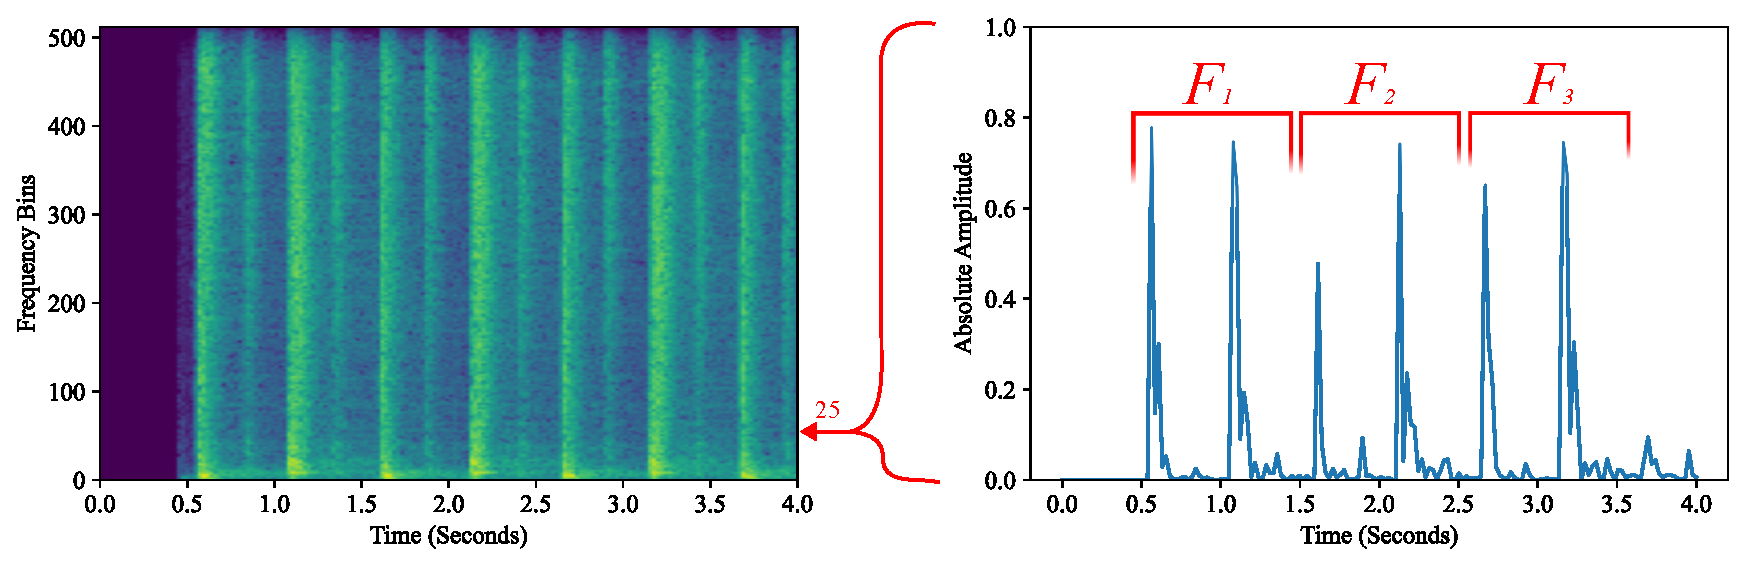
\includegraphics[width=\linewidth]{Figures/chap4/proposed/bj.eps}
    \caption{Illustration of repeating beats in the song "Billie Jean" by Michael Jackson\cite{michael_jackson_billie_1982} starting at the beginning.}
    \label{fig:billie-jean}
\end{figure}

\section{Main Idea}
\label{sec:idea}

To analyze the repeating signal easier, I focus on MDCT's 25th frequency bin which is shown on the right side of figure \ref{fig:billie-jean}. As can be seen in this Amplitude-Time plot, repeating drum sounds are visible as sudden spikes jumping from 0 to .8 in the amplitude. Knowing the song and seeing this plot, I can identify 3 repeating frames: first from 0.5 to 1.5 seconds ($F_1$), second from 1.5 to 2.5 seconds ($F_2$), and third from 2.5 to 3.5 seconds ($F_3$). As for a computer to identify matching frames, it can pick a frame (for example $F_3$) and loop through a shifting frame that is going backward in time while calculating the sum of absolute differences between these two frames. As can be seen in figure \ref{fig:shifting}, the output of this calculation has the minimum amount at 1 second. This means that the best candidate for $F_3$ to reuse is a frame starting 1 second earlier, i.e $F_2$.

\begin{figure}[ht] 
    \centering
    \includesvg[width=0.5\linewidth]{Figures/chap4/proposed/shift.svg}
    \caption{Sum of Absolute Differences between $F_3$ and a shifting frame going backwards in time.}
    \label{fig:shifting}
\end{figure}

The minimum amount in figure \ref{fig:shifting} is almost always not zero. That is because even though two audio signals sound identical to a human ear, they have some level of imperceptible differences. Figure \ref{fig:f3af2} shows these differences more clearly by overlapping both $F_3$ and $F_2$ on each other. When subtracting these two frames, as can be seen in figure \ref{fig:f3-f2}, the output is not zero, but it has some noises around the zero amplitude. This can be evidence of the reason the DEFLATE algorithm can not perform its lossless compression over songs with repeating notes because the repetition is not exact.

So because human ears can not perceive minor differences between $F_3$ and $F_2$, I propose that by manipulating signals we can help the DEFLATE algorithm and achieve a better compression size. This manipulation can be done by removing noises around the zero amplitude of differences between two frames using a threshold. Figure \ref{fig:f3-f2} shows this threshold should be able to separate perceptible differences from imperceptible ones. Applying this \textbf{Zero Threshold} would result in many zeros (figure \ref{fig:pframe3}) which can be useful for the DEFLATE algorithm to identify as a reusable signal. The resulting frame has similarities with P-Frames in the video encoding layer of MPEG-1 standard\cite{mpeg1-1993-video}.

\begin{figure}[ht]   
    \centering
    \begin{subfigure}{0.24\textwidth}
        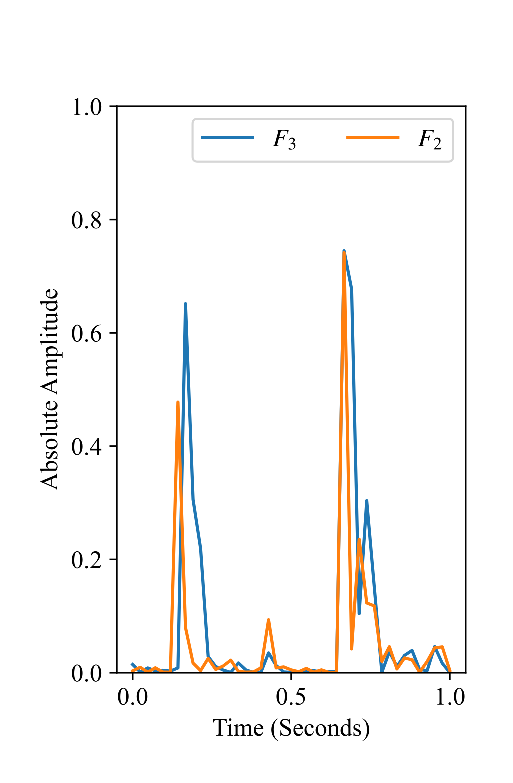
\includegraphics[width=\linewidth]{Figures/chap4/proposed/f3af2.eps}        
        \caption{$F_3$ and $F_2$}
        \label{fig:f3af2}
    \end{subfigure}
    \begin{subfigure}{0.24\textwidth}
        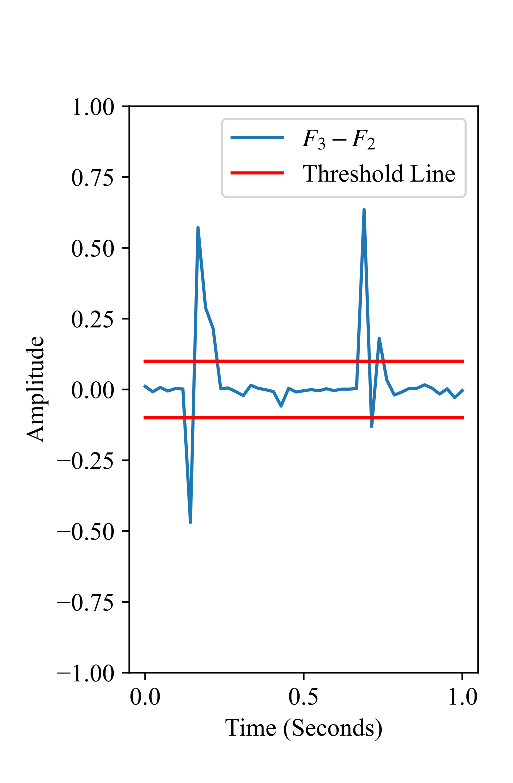
\includegraphics[width=\linewidth]{Figures/chap4/proposed/f3-f2.eps}        
        \caption{$F_3 - F_2$}
        \label{fig:f3-f2}
    \end{subfigure}
    \begin{subfigure}{0.24\textwidth}
        \includesvg[width=\linewidth]{Figures/chap4/proposed/pframe3.svg}
        \caption{$P_3$}
        \label{fig:pframe3}
    \end{subfigure}
    \begin{subfigure}{0.24\textwidth}
        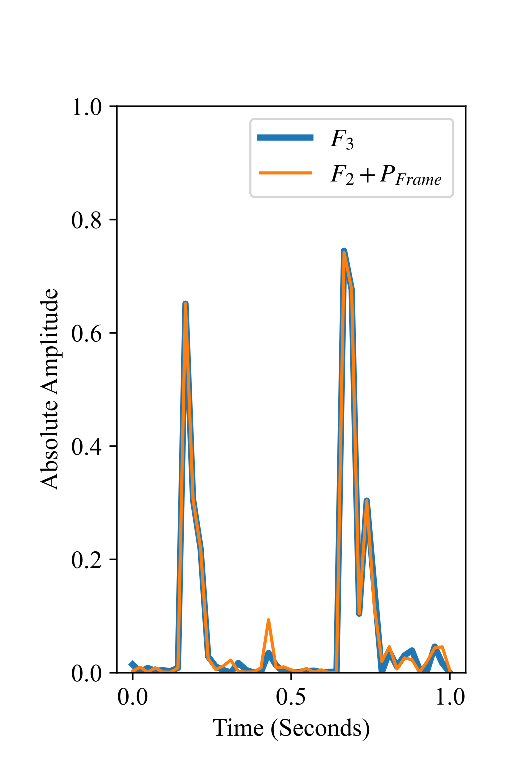
\includegraphics[width=\linewidth]{Figures/chap4/proposed/f3f2+p.eps}        
        \caption{$F_3$ and $F_2+P_3$}
        \label{fig:f3f2p}
    \end{subfigure}
    \caption{Illustration of P-Frame logic}
    \label{fig:pframe-logic}
\end{figure}

The rest of the properties of this audio compression idea are inspired by the MPEG-1 video encoder in which two types of frames are defined. \textbf{Intra-Frames or Independent-Frames (I-Frames)} are the ones that can be decoded independently and they contain a complete JPEG image. \textbf{Inter-Frames or Predicted-Frames (P-Frames)} are the ones that are dependent on another I-Frame or P-Frame to be decoded and they only contain the difference between the two images. 

So similar to the MPEG scheme, a frame that is made from the differences of audio frames can be named a P-Frame, while an independent audio frame can be named an I-Frame. The proposed encoding saves I-Frames alongside P-Frames. P-Frames also hold a number to indicate how many frames are they referring back in time while they are keeping only the differences between the frame at their place and the referred frame (as shown with arrows in figure \ref{fig:ipp}). The decoder would reconstruct frames by adding the referenced frame with the stored difference. Figure \ref{fig:f3f2p} shows the similarity of the original $F_3$ and the reconstructed signal. Obviously, the similarity between the original and the reconstructed signal is dependent on the threshold parameter. If the threshold parameter is chosen carelessly, it can produce perceptible differences in the decoded signal.

\begin{figure}[ht] 
    \centering
    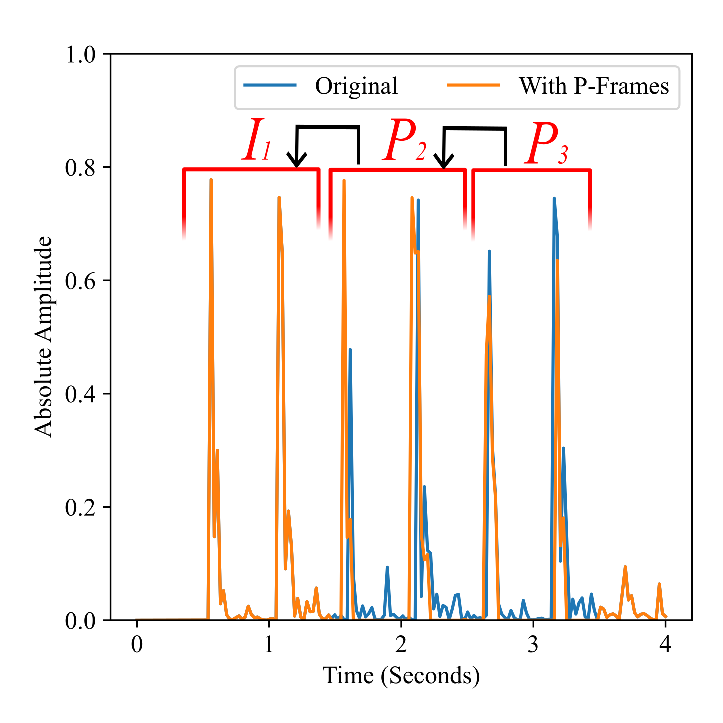
\includegraphics[width=0.5\linewidth, height=0.35\linewidth]{Figures/chap4/proposed/ipp.eps}
    \caption{Illustration of P-Frame logic and its comparison outcome with the original}
    \label{fig:ipp}
\end{figure}

To make this proposed approach more efficient, some conditions need to be defined, managed, and clarified:
\begin{itemize}
    \item A P-Frame should be used only if it has less information compared to the corresponding I-Frame. In cases where a repeating frame can not be found, using a P-Frame would contain a greater or equal amount of information and therefore it would not useful for the compression size. 
    \item Each decoding from a P-Frame produces a signal that is imperceptible compared to the original. However, after continuous use of P-Frames, all these minor imperceptible differences can accumulate to some quiet but perceptible noises. Therefore, similar to the MPEG scheme, I-Frames should be forced to be used on a constant frequency. The frequency of I-Frame enforcement can be called \textbf{I-Rate}. 
    \item It would be very inefficient to find a suitable similarity between two frames that are 1 minute apart. Finding a suitable reference for a P-Frame should have a limit. Without this limit, the processing time would increase exponentially. We can use the same I-Rate parameter and enforce P-Frames not to look further behind an enforced I-Frame.
    \item It is not efficient for a frame to have the size of 1 second. Even though the 1 second was used in the example above for simpler analysis, in fact, a smaller frame size can increase the chances of finding similarities. I propose that we use the smallest frame size possible which is one single MDCT time block or one single column of MDCT containing only 512 frequency bins. It an audio file with sample rate of 44.1 KHz, it would be the equavalent of .023 of a second ($= 1 / (44100 / 512 / 2)$).
    \item Because the frame size is proposed to be only one single MDCT columns, our frame comparisons will only be operating in the frequency domain and not the time domain. Therefore, even though the comparison method might be similar to the correlator or the matched filter, the comparison is fundamentally different because of the use of MDCT.
\end{itemize}

\section{Implementation}
\label{sec:implementation}

Algorithm \ref{alg:find-pframe} shows a function that is responsible to find a suitable P-Frame using the conditions mentioned above. It creates an I-Frame as a comparison to all shifting P-Frames and chooses the one that would create the most number of zeros. The function then returns the generated frame ($F$) and the relative reference of a frame that was used to generate it ($r$). If the function decides on using an I-Frame, it would use zero inside the $r$ variable.

\begin{algorithm}[ht]
\caption{Finding the most similar frames for the encoding (P-Frame)}
\label{alg:find-pframe}
\begin{algorithmic}
\Function{EncodeFrame}{$M_{t\times 512}, t, iRate, iThreshold, pThreshold$}
    \State $P \gets$ \Call{Zeros}{$iRate$}
    \State $F \gets$ \Call{Zeros}{$iRate, 512$}
    \\
    \State $N \gets$ \Call{Max}{$M[t]$}
    \State $F[0] \gets$ \Call{Threshold}{$M[t], iThreshold \times N$} \Comment{The I-Frame}
    \State $P[0] \gets$ \Call{Count\_Zeros}{$F_0$}
    \\
    \For{$i=1$ \textbf{to} $iRate$}
        \If{($t - i) \mod{iRate} = 0$}
            \State \textbf{break} \Comment{The I-Rate Limit}
        \EndIf
        \\
        \State $dF \gets M[t] - M[t - i]$
        \State $F[i] \gets$ \Call{Threshold}{$dF, pThreshold$} \Comment{P-Frames}
        \State $P[i] \gets$ \Call{Count\_Zeros}{$F[i]$}
    \EndFor
    \\
    \State $r \gets$ \Call{ArgMax}{$P$} \Comment{Pick the Best}
    \State \Return $(r, F[r])$
\EndFunction
\end{algorithmic}
\end{algorithm}

As can be seen in algorithm \ref{alg:scheme}, by calling the defined function repeatedly over the whole MDCT matrix, we can achieve a modified matrix of frames and an array of all used references. These two data structures can then be given to the DEFLATE algorithm to store on a hard drive. Later for decoding, these two data structures can be reconstructed back from DEFLATE and P-Frames, identifiable by their non-zero reference, can be changed back into I-Frames by summing the referenced frame with the P-Frame. Lastly, the matrix can use the inverse of MDCT to produce raw audio signals.

\begin{algorithm}[ht]
\caption{Proposed new P-Frame scheme}\label{alg:scheme}
\begin{algorithmic}
\Function{Encode}{$W, iRate, iThreshold, pThreshold$}
    \State $M_{t \times 512} \gets \Call{MDCT}{W}$
    \State $R_t \gets$ \Call{Zeros}{$t$}
    \For{$i=0$ \textbf{to} $t$}
        \State $R[i], M[i] \gets$ \Call{EncodeFrame}{$M, i, iRate, iThreshold, pThreshold$}
    \EndFor
    \State \Return \Call{Deflate}{$R$}, \Call{Deflate}{$M$}
\EndFunction
\\
\Function{Decode}{$Z_r, Z_m$}    
    \State $M_{t \times b} \gets$ \Call{Deflate$^{-1}$}{$Z_m$}
    \State $R_{t} \gets$ \Call{Deflate$^{-1}$}{$Z_r$}
    \For{$i=0$ \textbf{to} $t$}
        \If{$R[i] > 0$}
            \State $M[i] \gets M[i] + M[i-R[i]]$
        \EndIf
    \EndFor
    \State \Return \Call{MDCT$^{-1}$}{$M$}
\EndFunction
\end{algorithmic}
\end{algorithm}

\section{Exploration Tests}
\label{sec:tests}

Now with the new P-Frame scheme defined, it is time to observe how it behaves on our chosen example, the "Billie Jean" song. The parameters that I used were: 2 seconds for I-Rate, $10^{-3}$ for P-Frame Threshold, and 0 for I-Frame Threshold. Looking at the histogram of generated references in figure \ref{fig:hist}, it can be seen that more than 98\% of frames were chosen to be P-Frames ($h(0)=1.5\%$) which means for each one of them, at least one element (2 bytes) became zero and helped to improve the compression. Interestingly, the histogram seems to be having jumps around 44 frames (1 second), 33 frames (.75 of a second), 22 frames (.5 of a second), and 11 frames (.25 of a second). This means that the algorithm is able to find the 1-second repeating beats and fractions of it based on the song's $4/4$ time signature. 

\begin{figure}[ht] 
    \centering
    \includesvg[width=0.5\linewidth]{Figures/chap4/tests/hist.svg}
    \caption{Histogram of References from P-Frame encoding over the song "Billie Jean" by Michael Jackson}
    \label{fig:hist}
\end{figure}

Most noticeably in Figure \ref{fig:hist}, we can see that more than 13.2\% of P-Frames refer to their most immediate previous frame ($\sim .023$ of a second) and more than 5\% refer to their second most immediate previous frame ($\sim .045$ of a second). This probably means even though repeating beats and notes can have similar frames, those frames related to the same note are even more similar. Looking at the differences between I-Frame only and P-Frame spectrum in figure \ref{fig:billie_jean_25sec}, we can see that \ref{fig:saved_25sec} has darker areas compared to the \ref{fig:unmodified_25sec}, especially in areas that the drum sound is decaying and the red line is higher. The red line shows the increase in the number of zero elements that were added after applying the P-Frame scheme. This is an indication of how many bytes were saved and more compression each P-Frame.

Looking at the used references in Figure \ref{fig:ref_25sec}, we can see that between 0 to 2 seconds, the distance of references increases linearly except for areas where an unfamiliar or new signal is played. At 2 seconds, because the parameter I-Rate was set, references suddenly drop to zero and they would not refer to any frames before 2 seconds. This will be repeated every 2 seconds.

\begin{figure}[ht]
\centering
\begin{subfigure}{0.30\textwidth}
    \includesvg[width=\linewidth]{Figures/chap4/tests/billie_jean_2.5sec.svg}
    \caption{I-Frames Only}
    \label{fig:unmodified_25sec}
\end{subfigure}
\hfill
\begin{subfigure}{0.32\textwidth}
    \includesvg[width=\linewidth]{Figures/chap4/tests/saved_2.5sec.svg}
    \caption{P-Frames \& Increased Number of Zero Elements}
    \label{fig:saved_25sec}
\end{subfigure}
\hfill
\begin{subfigure}{0.32\textwidth}
    \includesvg[width=\linewidth]{Figures/chap4/tests/ref_2.5sec.svg}
    \caption{P-Frames \& References}
    \label{fig:ref_25sec}
\end{subfigure}
\caption{Effectiveness of P-Frames over the drums in the beginning song "Billie Jean" by Michael Jackson}
\label{fig:billie_jean_25sec}
\end{figure}

In a different part of the song where more musical instruments are being played and Michael Jackson starts singing, we can see in figure \ref{fig:saved_3sec} shows less increase in the number of zero elements as compared to \ref{fig:unmodified_3sec}. Expectedly, at 29.5 seconds where vocal signals seem to look more chaotic and less repetitive, we can see that the algorithm has failed to find similarities with previous frames. Similarly, in figure \ref{fig:ref_3sec}, we can see that the distance of references suddenly drops at 29.5 seconds before I-Rate enforces an I-Frame at 30 seconds. This would be an indication that the P-Frame schema behaves differently in different parts of music depending on its ability to detect and reuse similar or repeated information.

\begin{figure}[ht]
\centering
\begin{subfigure}{0.30\textwidth}
    \includesvg[width=\linewidth]{Figures/chap4/tests/billie_jean_3sec.svg}
    \caption{I-Frames Only}
    \label{fig:unmodified_3sec}
\end{subfigure}
\hfill
\begin{subfigure}{0.32\textwidth}
    \includesvg[width=\linewidth]{Figures/chap4/tests/saved_3sec.svg}
    \caption{P-Frames \& Increased Number of Zero Elements}
    \label{fig:saved_3sec}
\end{subfigure}
\hfill
\begin{subfigure}{0.32\textwidth}
    \includesvg[width=\linewidth]{Figures/chap4/tests/ref_3sec.svg}
    \caption{P-Frames \& References}
    \label{fig:ref_3sec}
\end{subfigure}
\caption{Effectiveness of P-Frames over the vocals in the song "Billie Jean" by Michael Jackson}
\label{fig:billie_jean_3sec}
\end{figure}

Overall, with the specified parameters, the P-Frame encoder is able to compress the "Billie Jean" song by more than 89.5 \% as compared to the lossless I-Frame scheme which is 95.1 \%. Because no other perceptual techniques were active, this means the P-Frame scheme alone has a 5.6 \% improvement in compression ratio. Evaluating the perceptual audio quality of the decoded signal, I got -.858 for the objective difference degree which means the difference between the original and the decoded signal is hard to perceive by the human ears.

The aforementioned results for this specific example indicate that the new approach is feasible and does a good job of compressing "Billie Jean"  song. Moreover, more songs are required to be tested and analyzed in order to consider these results more generally applicable. To investigate this, I run the P-Frame scheme on a larger dataset and I analyze these results statistically in chapter \ref{chapter:Exp}.
    \startchapter{Experiments}
\label{chapter:Exp}

In this chapter, I try to answer the research question: Can the described P-Frame schema improve the compression of pieces of music with repeated instrumental tones without adding perceptible differences? My hypothesis is that by reusing portions of audio that are being repeated (P-Frames), as long as a piece of music has repeating structure, the scheme should be able to compress better as compared to the compression of every single frame individually (I-Frames). Therefore, to answer the research question quantitatively, it is required to have a statistical analysis of numerical outputs (Dependent Variables) of the scheme that is run over a random collection of pieces of music while controlling all different variables to isolate our conditions (Independent Variables). The following describes my experimental design:

\begin{description}
\item[Population:] To have an unbiased and random set of pieces of music, I used the "test" set in MUSDB-HQ which consists of 50 full-length songs ($\sim$3h duration) with different genres along with their isolated drums, bass, vocals and others stems \cite{musdb18-hq}.

\item[Dependent Variables (DVs):] After running the compression scheme on each audio file, I measure the following:
\begin{itemize}
\item\textbf{Audio Quality:} the audio quality was measured using Objective Difference Grade (ODG) of Perceptual Evaluation of Audio Quality (PEAQ) \cite{peaq} to ensure that the compression scheme does not add perceptible artifacts. The range is between 0 and -4.
\item\textbf{Compression Ratio:} As each song has a different length, the output size of files is compared by measuring the ratio, so the range is between 0 and 1. It is calculated as:  Compressed File Size / Uncompressed File Size
\item\textbf{Desirability:} As ODG and Compression-Ratio are correlated, I need a new variable that can help me interpret the effectiveness of the scheme. This measure is named Desirability, has a range between 0 and -1, and is calculated as: (ODG/4) / Compression Ratio
\item\textbf{P-Ratio:} To measure the number of frames that are reused in the compressed file. P-Ratio has a range between 0 and 1 and is calculated as: N(used P-Frames) / N(all frames)
% \item MAYBE NOT NEEDED: Reference Distance Histogram represented in 25\%, 50\%, and 75\% quantiles.
\end{itemize}

\item[Control Variables:] To ensure that we measure only the effectiveness of reused frames, all other techniques of audio compression should be disabled and non-zero parameters should be set to the lowest amount. Therefore, after running the MDCT algorithm, the following parameters are used:
\begin{itemize}
\item\textbf{High Frequency Cut} = 0
\item\textbf{Rounding Decimals} = 0
\item\textbf{P-Frame Zero Threshold} = ${10}^{-5}$; this value can not be zero. So because MDCT numbers are between -1 and 1 with 12 digits of decimal points, we use the mentioned small value.
\item\textbf{I-Frame Zero Threshold} = ${10}^{-5}$; to be equal to the other threshold.
\item\textbf{I-Rate} = 2 seconds; Only in section \ref{sec:pframe-exp}.
\end{itemize}

\item[Independent Variables (IVs):] The following variables are purposely set and the scheme is executed once per each of them. So each song is compressed 42 ($=6\times 3 + 6\times 4$) times.
\begin{itemize}[leftmargin=*]
\item\textbf{Audio Type} (6 levels)
\begin{enumerate}[nosep, leftmargin=*]
\item\textbf{Mixture:} The original song including vocals, drums, and the rest of the instruments.
\item\textbf{Vocals:} Only the vocal sound of the song which normally doesn't have repeating tones.
\item\textbf{Drums:} Only the drums sound of the song which normally repeats with the beat.
\item\textbf{REPET's Foreground:} The masked foreground of the REPET algorithm which is determined based on lack of repetition.
\item\textbf{REPET's Background:} The masked background of the REPET algorithm which is determined based on having repetitions.
\item\textbf{Sum:} A mixture of the latter two which holds the concatenation of REPET's foreground with only I-Frames and REPET's background with P-Frames.
\end{enumerate}
\item\textbf{Scheme} (3 levels); Only used in section \ref{sec:pframe-exp}.
\item\textbf{I-Rate} (4 levels); Only used in section \ref{sec:i-rates}.
\end{itemize}

\item[Statistical Analysis:] For each DV, I provide figures that show the mean of outputs in each one of the IVs ($N=50$). Error bars in graphs are all showing 95\% confidence intervals. In addition to the graphs, descriptive and inferential statistics are provided. Data is analyzed using a 2-way repeated-measures ANOVA and Tukey HSD post-hoc test. For every ANOVA test, the assumptions of Normality and Sphericity of Distributions were checked. Despite some mild violations of Normality, there was no violation of the Sphericity test. This means degrees of freedom never needed to be corrected. As for violations of the Normality test, it is believed that the ANOVA test is robust in groups of the same size.

\end{description}


\section{Effects of I-Rate on the Compression Scheme}
\label{sec:i-rates}

As described in section \ref{sec:idea}, the I-Rate parameter is the rate of forced I-Frames that P-Frames are not allowed to refer to any frame before them. A larger number in the I-Rate means P-Frames are allowed to look more back in time to find a suitable referenced frame to reuse. Additionally, it means more comparisons and more CPU time. In this section, I try to answer the question: What is the suitable amount of time for P-Frames to look back? My hypothesis is that, in the worst case, beats are repeated once per second. Therefore, 2 seconds for the I-Rate should be sufficient and there is no point in going back more in time to find a reference.

To test this hypothesis, DVs are measured as described at the beginning of chapter \ref{chapter:Exp} with an additional 4-level IV named I-Rates: 0.1 of a second, 1 second, 2 seconds, and 5 seconds. The following sections are reports for each measured variable.

\subsection{Audio Quality}

\begin{figure}[ht]
  \includesvg[inkscapelatex=false,  width=\linewidth]{Figures/chap5/irate-peaq.svg}
  \caption[Comparison of Audio Quality in different types of audio and I-Rates.]{Comparison of Audio Quality in different types of audio and I-Rates. Audio Quality is measured using Objective Difference Grade (ODG) in Perceptual Evaluation of Audio Quality (PEAQ) (0 = Imperceptible, -1 = Perceptible, but not annoying)}
  \label{fig:irate-peaq}
\end{figure}

It can be seen in Figure \ref{fig:irate-peaq} that mixture audio input is imperceptible in I-Rates of 0.1 of a second ($M=.15, SD=.037$), 1 second ($M=.125, SD=.099$), 2 seconds ($M=.114, SD=.137$), and 5 seconds ($M=.105, SD=.166$).
Similarly, REPET's background is imperceptible in I-Rates of 0.1 of a second ($M=.143, SD=.039$), 1 second ($M=.112, SD=.098$), 2 seconds ($M=.098, SD=.165$), and 5 seconds ($M=.089, SD=.187$).
Identically, the sum audio input is imperceptible in I-Rates of 0.1 of a second ($M=.148, SD=.038$), 1 second ($M=.121, SD=.107$), 2 seconds ($M=.111, SD=.148$), and 5 seconds ($M=.104, SD=.167$).
In REPET's foreground, however, the audio quality is slightly reduced with the increment of I-Rate from 0.1 of a second ($M=.092, SD=.064$), to 1 second ($M=-.036, SD=.185$), 2 seconds ($M=-.065, SD=.194$), and 5 seconds ($M=-.107, SD=.25$).
In drums audio, the audio quality is also slightly reduced with an I-Rate of 0.1 of a second ($M=.051, SD=.187$), to 1 second ($M=-.111, SD=.41$), and 2 seconds ($M=-.161, SD=.479$). Then it stays the same for the I-Rate of 5 seconds ($M=-.162, SD=.464$).
Most noticeably, the audio quality is highly reduced with the increment of I-Rate from 0.1 of a second ($M=.014, SD=.18$), to 1 second ($M=-.349, SD=.513$), 2 seconds ($M=-.46, SD=.645$), and 5 seconds ($M=-.603, SD=.805$).

Running further statistical analysis,  within-subject ANOVA showed that the audio quality is significantly affected by the used input audio type ($F(5,245)=31.4, p<.000, \eta_{p}^{2}=.39$), the I-Rate ($F(3,147)=44.8, p<.000, \eta_{p}^{2}=.477$), and the interaction between them ($F(15,735)=18.7, p<.000, \eta_{p}^{2}=.276$).
Tukey HSD post-hoc showed that the audio quality is significantly higher in I-Rate of 0.1 of a second ($M=.1, SD=.122$), as compared to other used I-Rates (all $p$s $<.001$) while it showed no significant reduction of audio quality for the I-Rate of 1 second ($M=-.023, SD=.333$), 2 seconds ($M=-.06, SD=.407$), and 5 seconds ($M=-.096, SD=.479$). In vocals specifically, Tukey HSD showed no significant reduction of audio quality between I-Rates of 1 second and 2 seconds, and I-Rates of 2 seconds and 5 seconds. However, the audio quality between I-Rates of 1 second and 5 seconds are significantly lowered ($p=.011$).

In summary, the results confirmed that, except for vocals, the lossy compression remains imperceptible with any amount of I-Rate and it stabilizes when it is higher than 1 second.

\subsection{Compression Ratio}

\begin{figure}[ht]
  \includesvg[inkscapelatex=false,  width=\linewidth]{Figures/chap5/irate-compression-ratio.svg}
  \caption{Comparison of Compression Ratio in different types of audio and I-Rates}
  \label{fig:irate-compression-ratio}
\end{figure}

It can be seen in Figure \ref{fig:irate-compression-ratio} that mixture audio input is slightly compressed in I-Rate of 0.1 of a second ($M=.898, SD=.025$), and a bit more in 1 second ($M=.875, SD=.034$), 2 seconds ($M=.873, SD=.035$), and 5 seconds ($M=.871, SD=.036$).
Similarly, drum audio input is slightly compressed in I-Rate of 0.1 of a second ($M=.804, SD=.105$), and a bit more in 1 second ($M=.761, SD=.122$), 2 seconds ($M=.755, SD=.125$), and 5 seconds ($M=.751, SD=.126$). 
Identically, REPET's foreground audio input is slightly compressed in I-Rate of 0.1 of a second ($M=.834, SD=.042$), and a bit more in 1 second ($M=.78, SD=.053$), 2 seconds ($M=.774, SD=.054$), and 5 seconds ($M=.768, SD=.055$).
As for REPET's background, the audio input is slightly compressed in I-Rate of 0.1 of a second ($M=.88, SD=.027$), and a bit more in 1 second ($M=.855, SD=.037$), 2 seconds ($M=.852, SD=.038$), and 5 seconds ($M=.85, SD=.039$).
The sum audio input is also slightly compressed in I-Rate of 0.1 of a second ($M=.859, SD=.032$), and a bit more in 1 second ($M=.847, SD=.037$), 2 seconds ($M=.846, SD=.037$), and 5 seconds ($M=.844, SD=.038$).
Most noticeably, vocal audio input is compressed more than the other with the increment of I-Rate from 0.1 of a second ($M=.643, SD=.17$), to 1 second ($M=.598, SD=.174$), 2 seconds ($M=.594, SD=.174$), and 5 seconds ($M=.589, SD=.174$).

Running further statistical analysis,  within-subject ANOVA showed that Compression Ratio is significantly affected by the used input audio type ($F(5,245)=72.4, p<.000, \eta_{p}^{2}=.596$), the I-Rate ($F(3,147)=292, p<.000, \eta_{p}^{2}=.856$), and the interaction between them ($F(15,735)=48, p<.000, \eta_{p}^{2}=.495$).
Tukey HSD post-hoc showed that the compression is significantly worse in I-Rate of 0.1 of a second ($M=.82, SD=.12$), as compared to other used I-Rates (all $p$s $<.001$) while it showed no significant improvement of compression for the I-Rate of 1 second ($M=-.786, SD=.131$), 2 seconds ($M=.782, SD=.133$), and 5 seconds ($M=.779, SD=.134$). 
In vocals specifically, Tukey HSD showed no significant reduction of audio quality in I-Rates of 0.1 of a second, 1 second, 2 seconds and 5 seconds (all $p$s $>.319$).

In summary, the results confirmed that the Compression Ratio doesn't improve with I-Rates higher than 1 second.

\subsection{Desirability}

\begin{figure}[ht]
  \includesvg[inkscapelatex=false,  width=\linewidth]{Figures/chap5/irate-desirable.svg}
  \caption{Comparison of Desirability in different types of audio and I-Rates}
  \label{fig:irate-desirable}
\end{figure}

It can be seen in Figure \ref{fig:irate-desirable} that mixture audio input is the most desirable with I-Rate of 0.1 of a second ($M=.042, SD=.01$), 1 second ($M=.035, SD=.029$), 2 seconds ($M=.032, SD=.041$), and 5 seconds ($M=.03, SD=.05$).
Similarly, REPET's background is highly desirable with I-Rates of 0.1 of a second ($M=.041, SD=.011$), 1 second ($M=.032, SD=.034$), 2 seconds ($M=.028, SD=.051$), and 5 seconds ($M=.026, SD=.059$).
Identically, the sum audio input is desirable with I-Rates of 0.1 of a second ($M=.043, SD=.011$), 1 second ($M=.036, SD=.033$), 2 seconds ($M=.032, SD=.045$), and 5 seconds ($M=.031, SD=.051$).
In REPET's foreground, however, the increment of I-Rate makes the result slightly less desirable from 0.1 of a second ($M=.028, SD=.02$), to 1 second ($M=-.012, SD=.063$), 2 seconds ($M=-.022, SD=.065$), and 5 seconds ($M=-.036, SD=.086$).
In drums audio, Desirability is also being slightly reduced with an I-Rate of 0.1 of a second ($M=.012, SD=.068$), to 1 second ($M=-.051, SD=.173$), and 2 seconds ($M=-.07, SD=.205$). Then it stays almost the same for the I-Rate of 5 seconds ($M=-.066, SD=.18$).
Most noticeably, in vocals, the increment of I-Rate makes the algorithm least desirable from 0.1 of a second ($M=.006, SD=.072$), to 1 second ($M=-.205, SD=.368$), 2 seconds ($M=-.241, SD=.36$), and 5 seconds ($M=-.342, SD=.563$).

Running further statistical analysis,  within-subject ANOVA showed that audio quality is significantly affected by the used input audio type ($F(5,245)=21.8, p<.000, \eta_{p}^{2}=.308$), the I-Rate ($F(3,147)=28.5, p<.000, \eta_{p}^{2}=.368$), and the interaction between them ($F(15,735)=12.6, p<.000, \eta_{p}^{2}=.205$).
Tukey HSD post-hoc showed that the Desirability is significantly higher in I-Rate of 0.1 of a second ($M=.029, SD=.044$), as compared to other used I-Rates (all $p$s $<.001$) while it showed no significant reduction of Desirability for the I-Rate of 1 second ($M=-.028, SD=.189$), 2 seconds ($M=-.04, SD=.198$), and 5 seconds ($M=-.06, SD=.278$). In vocals specifically, Tukey HSD showed no significant reduction of Desirability between I-Rates of 1 second and 2 seconds, and I-Rates of 2 seconds and 5 seconds. However, the I-Rate of 5 seconds is significantly less desired than the I-Rate of 1 second ($p=.02$).

In summary, the results confirmed that, except for vocals, the lossy compression remains desirable with any amount of I-Rate and it stabilizes when it is higher than 1 second.

\subsection{P-Ratio}

\begin{figure}[ht]
  \includesvg[inkscapelatex=false,  width=\linewidth]{Figures/chap5/irate-pratio.svg}
  \caption{Comparison of P-Ratios in different types of audio and I-Rates}
  \label{fig:irate-pratio}
\end{figure}

It can be seen in figure \ref{fig:irate-pratio} that in mixture audio input, P-Ratio starts with a lower value in 0.1 of a second ($M=.737, SD=.014$), and then it increases in 1 second ($M=.961, SD=.019$), 2 seconds ($M=.972, SD=.019$), and 5 seconds ($M=.979, SD=.019$).
Similarly in REPET's foreground, P-Ratio starts with a lower value in 0.1 of a second ($M=.72, SD=.019$), and then it increases in 1 second ($M=.938, SD=.025$), 2 seconds ($M=.949, SD=.026$), and 5 seconds ($M=.956, SD=.026$).
Identically in both REPET's background and the sum audio input, P-Ratio also starts with a lower value in 0.1 of a second ($M=.737, SD=.015$), and then it increases in 1 second ($M=.96, SD=.019$), 2 seconds ($M=.972, SD=.019$), and 5 seconds ($M=.978, SD=.02$).
In drums audio input, P-Ratio was slightly lower compared to the former in 0.1 of a second ($M=.687, SD=.075$), and then it increases in 1 second ($M=.895, SD=.098$), 2 seconds ($M=.906, SD=.099$), and 5 seconds ($M=.912, SD=.1$).
Most noticeably in vocals, P-Ratio was highly lower compared to the former in 0.1 of a second ($M=.58, SD=.155$), and then it increases in 1 second ($M=.756, SD=.202$), 2 seconds ($M=.765, SD=.204$), and 5 seconds ($M=.77, SD=.206$).

Running further statistical analysis,  within-subject ANOVA showed that P-Ratio is significantly affected by the used input audio type ($F(5,245)=40.6, p<.000, \eta_{p}^{2}=.453$), the I-Rate ($F(3,147)=20263, p<.000, \eta_{p}^{2}=.998$), and the interaction between them ($F(15,735)=40.6, p<.000, \eta_{p}^{2}=.453$).
Tukey HSD post-hoc showed that P-Ratio is significantly lower in I-Rate of 0.1 of a second ($M=.7, SD=.09$), as compared to other used I-Rates (all $p$s $<.001$) while it showed no significant improvement for the I-Rate of 1 second ($M=.912, SD=.118$), 2 seconds ($M=.923, SD=.119$), and 5 seconds ($M=.929, SD=.12$). Moreover, Tukey HSD showed that P-Ratio is significantly lower in vocals ($M=.718, SD=.207$), as compared to other used I-Rates (all $p$s $<.001$) while it showed no significant change for the mixture ($M=-.912, SD=.103$), drums ($M=.85, SD=.132$), REPET's foreground ($M=.891, SD=.102$), REPET's background ($M=.912, SD=.103$), and the sum ($M=.912, SD=.103$).

In summary, the results confirmed that, except for vocals, the lossy compression can find P-Frames with any amount of I-Rate and it stabilizes when it is higher than 1 second.

% \subsection{Reference Distance}

% \begin{figure}[ht]
%   \includesvg[inkscapelatex=false,  width=\linewidth]{Figures/chap5/irate-quantiles.svg}
%   \caption{Comparison of Reference Distances in different types of audio and I-Rates}
%   \label{fig:irate-quantiles}
% \end{figure}

% \TODO{Text needed for reference distance} 
\section{Comparison of Compression Schemas}
\label{sec:pframe-exp}

It can be concluded from section \ref{sec:i-rates} that 2 seconds is a suitable value to use for the I-Rate parameter and we only use this constant value for the P-Frame schema. Now it is time to answer the main research question: i.e "Can the described P-Frame schema improve the compression of pieces of music with repeated instrumental tones without adding perceptible differences?". To study the answer, DVs are measured as described at the beginning of chapter \ref{chapter:Exp} with an additional 3-level IV named \textbf{Schema}:

\begin{enumerate}
\item\textbf{Lossless:} The base condition which saves raw MDCT output.
\item\textbf{Only I-Frames:} The MDCT output with all I-Frames zero thresholds applied.
\item\textbf{With P-Frames:} The proposed new compression scheme.
\end{enumerate}

\noindent Following sections are reports for each measured variable.

\subsection{Audio Quality}

\begin{figure}[ht]
  \includesvg[inkscapelatex=false,  width=\linewidth]{Figures/chap5/input-peaq.svg}
  \caption[Comparison of Schemas in Audio Quality amongst different types of audio]{Comparison of Schemas in Audio Quality amongst different types of audio. Audio Quality is measured using Objective Difference Grade (ODG) in Perceptual Evaluation of Audio Quality (PEAQ) (0 = Imperceptible, -1 = Perceptible, but not annoying)}
  \label{fig:input-peaq}
\end{figure}

\begin{table}[ht]
\fontsize{8}{10}\selectfont
\newcommand{\wrap}[1]{\parbox{2cm}{\vspace{1.5mm}#1\vspace{1mm}}}
\centering
\begin{tabularx}{\linewidth}{|m{2cm}||Y|Y||Y|Y||Y|Y||Y|Y||Y|Y|}
\hline
Input Type & \multicolumn{2}{c||}{Mixture} & \multicolumn{2}{c||}{Vocals} & \multicolumn{2}{c||}{Drums} & \multicolumn{2}{c||}{\wrap{REPET's\\ Foreground}} & \multicolumn{2}{c|}{\wrap{REPET's\\ Background}} \\
\hline
& Mean & SD & Mean & SD & Mean & SD & Mean & SD & Mean & SD \\
\hline
Lossless & .164 & .009 & .151 & .015 & .149 & .03 & .15 & .016 & .159 & .009 \\
\hline
All I-Frames & .152 & .035 & .146 & .017 & .113 & .088 & .14 & .022 & .146 & .039 \\
\hline
With P-Frames & .114 & .137 & -.46 & .645 & -.161 & .479 & -.065 & .194 & .098 & .165\\
\hline
\end{tabularx}
\caption[Table of Schemas in Audio Quality amongst different types of audio]{Table of Schemas in Audio Quality amongst different types of audio. Audio Quality is measured using Objective Difference Grade (ODG) in Perceptual Evaluation of Audio Quality (PEAQ) (0 = Imperceptible, -1 = Perceptible, but not annoying)}
\label{tab:input-peaq}
\end{table}

It can be seen in figure \ref{fig:input-peaq} and table \ref{tab:input-peaq} that lossless encoding has an ODG above zero (imperceptible) and very similar in all input types.
Similarly, all I-frame encoding is imperceptible with a slight decrease in audio quality in all input types.
However, with P-frame encoding can have an ODG below zero depending on the audio type with even more decrease in all input types.

Within-subject ANOVA showed that the audio quality is significantly affected by the type of audio  ($F(4,196)=24.4, p<.000, \eta_{p}^{2}=.332$), the used schema ($F(2,98)=56.4, p<.000, \eta_{p}^{2}=.535$), and the interaction between them ($F(8,392)=25.1, p<.000, \eta_{p}^{2}=.339$).
Tukey HSD post-hoc showed that the audio quality for vocals ($M=-.054, SD=.469$) was significantly lower than mixture ($M=.144, SD=.083$), drums ($M=.033, SD=.313$), REPET's foreground ($M=.075, SD=.15$), and REPET's background ($M=.134, SD=.1$), (all $p$s $<.007$).
Beside that, the audio quality for drums was significantly lower than the mixture, and REPET's background (all $p$s $<.001$).
It is important to mention that Tukey HSD showed no significant reduction of audio quality for having P-frames ($M=-.06, SD=.407$), all I-frames ($M=.139, SD=.049$), and lossless ($M=.155, SD=.018$).

In summary, the results confirmed that having P-Frames can significantly reduce the audio quality on vocals, and not the background sounds such as drums. However, it might be confusing why mixtures have a better sound quality with P-Frames scheme as compared to drums. This can probably be because drums audio type contains more silence and human ears can perceive differences in silence better as compared to the mixture with many accompanying instruments.

\subsection{Compression Ratio}

\begin{figure}[ht]
  \includesvg[inkscapelatex=false,  width=\linewidth]{Figures/chap5/input-compression-ratio.svg}
  \caption{Comparison of Schemas in Compression Ratio amongst different types of audio}
  \label{fig:input-compression}
\end{figure}

\begin{table}[ht]
\fontsize{8}{10}\selectfont
\newcommand{\wrap}[1]{\parbox{2cm}{\vspace{1.5mm}#1\vspace{1mm}}}
\centering
\begin{tabularx}{\linewidth}{|m{2cm}||Y|Y||Y|Y||Y|Y||Y|Y||Y|Y|}
\hline
Input Type & \multicolumn{2}{c||}{Mixture} & \multicolumn{2}{c||}{Vocals} & \multicolumn{2}{c||}{Drums} & \multicolumn{2}{c||}{\wrap{REPET's\\ Foreground}} & \multicolumn{2}{c|}{\wrap{REPET's\\ Background}} \\
\hline
& Mean & SD & Mean & SD & Mean & SD & Mean & SD & Mean & SD \\
\hline
Lossless & .993 & .019 & .717 & .182 & .85 & .123 & .91 & .026 & .917 & .021 \\
\hline
All I-Frames & .906 & .023 & .704 & .178 & .836 & .124 & .839 & .04 & .893 & .021 \\
\hline
With P-Frames & .873 & .035 & .594 & .174 & .755 & .125 & .774 & .054 & .893 & .022 \\
\hline
\end{tabularx}
\caption{Table of Schemas in Compression Ratio amongst different types of audio}
\label{tab:input-compression}
\end{table}

It can be seen in figure \ref{fig:input-compression} and table \ref{tab:input-compression} that lossless encoding has a very similar compression ratio in the mixture, REPET's foreground, and REPET's background.
However, lossless encoding had a lower compression ratio in the vocals, and drums.
Compared to the lossless encoding, fully I-frame encoding reduced the compression ratio in all input types.
Having P-frames reduced the compression ratio even further in all input types.
Within-subject ANOVA showed that compression ratio is significantly affected by the used input audio type ($F(4,196)=51.8, p<.000, \eta_{p}^{2}=.514$), the used schema ($F(2,98)=164, p<.000, \eta_{p}^{2}=.77$), and the interaction between them ($F(8,392)=20.3, p<.000, \eta_{p}^{2}=.293$).
Tukey HSD post-hoc showed that the compression ratio with P-frame encoding ($M=-.782, SD=.133$) was significantly lower than the compression ratio for fully I-frame encoding ($M=.836, SD=.122, p<.0001$), while the fully I-frame encoding was not significantly lower than the lossless encoding ($M=.033, SD=.313, p=1$).
As for audio inputs, Tukey HSD post-hoc showed that the compression ratio for vocals ($M=.672, SD=.185$) was significantly lower than the compression ratio for mixture ($M=.904, SD=.036$), drums ($M=.814, SD=.13$), REPET's foreground ($M=.841, SD=.07$), and REPET's background ($M=.888, SD=.039$).
Beside that, the compression ratio for drums was significantly lower than the compression ratio for mixture, REPET's foreground, and REPET's background (all $p$s $<.0005$).
However, the compression ratio for drums was not significantly different than REPET's foreground ($p=154$). Similarly, the compression ratio for the mixture was not significantly different than the compression ratio for REPET's background ($p=696$).

In summary, the results confirmed that having P-Frames can significantly reduce the compression ratio.
Furthermore, the compression ratio is highly dependent on the type of input audio. Specifically, having more silence in the audio input will reduce the compression ratio.
This explains the reason that vocals and drums audio inputs have better compression ratios.

\subsection{Desirability}

\begin{figure}[ht]
  \includesvg[inkscapelatex=false,  width=\linewidth]{Figures/chap5/input-desirable.svg}
  \caption{Comparison of Compression Schemas in Desirability amongst different types of audio}
  \label{fig:input-desirable}
\end{figure}

\begin{table}[ht]
\fontsize{8}{10}\selectfont
\newcommand{\wrap}[1]{\parbox{2cm}{\vspace{1.5mm}#1\vspace{1mm}}}
\centering
\begin{tabularx}{\linewidth}{|m{2cm}||Y|Y||Y|Y||Y|Y||Y|Y||Y|Y|}
\hline
Input Type & \multicolumn{2}{c||}{Mixture} & \multicolumn{2}{c||}{Vocals} & \multicolumn{2}{c||}{Drums} & \multicolumn{2}{c||}{\wrap{REPET's\\ Foreground}} & \multicolumn{2}{c|}{\wrap{REPET's\\ Background}} \\
\hline
& Mean & SD & Mean & SD & Mean & SD & Mean & SD & Mean & SD \\
\hline
Lossless & .044 & .003 & .059 & .033 & .045 & .012 & .041 & .005 & .043 & .003 \\
\hline
All I-Frames & .042 & .01 & .058 & .03 & .034 & .027 & .042 & .007 & .041 & .011 \\
\hline
With P-Frames & .032 & .041 & -.241 & .36 & -.07 & .205 & -.022 & .065 & .028 & .051\\
\hline
\end{tabularx}
\caption{Table of Compression Schemas in Desirability amongst different types of audio}
\label{tab:input-desirable}
\end{table}

It can be seen in figure \ref{fig:input-desirable} and table \ref{tab:input-desirable} that desirability is not much being reduced in mixture and REPET's background audio inputs with all compression schemes.
However, with P-frame encoding, desirability is slightly reduced in drums and REPET's foreground audio and it is reduced the most in vocals audio input.
Within-subject ANOVA showed that desirability is significantly affected by the used input audio type ($F(4,196)=16.3, p<.000, \eta_{p}^{2}=.25$), the used schema ($F(2,98)=46.7, p<.000, \eta_{p}^{2}=.488$), and the interaction between them ($F(8,392)=21.9, p<.000, \eta_{p}^{2}=.309$).
Tukey HSD post-hoc showed that the desirability was significantly reduced in vocals with P-frame encoding and in drums with P-frame encoding compared to all other cases (all $p$s $<.0008$). However, the desirability of having P-frames is not significantly reduced in the mixture, REPET's foreground, and REPET's background.

In summary, the results confirmed that having P-frames can be significantly undesirable in vocals. Having P-frames can also significantly reduce desirability in drums but the mean difference shows it is not as undesirable as it is for vocals.

\section{Conclusions of Experiments} 

% \TODO{Write a summary of the main conclusions of the experiments - essentially repeat in condensed form the In summary sentences of the subsections in the chapter} 

To summarize, it can be concluded from section \ref{sec:i-rates} that 2 seconds is a suitable value to use for the I-Rate parameter for the P-Frame schema. Afterwards, from section \ref{sec:pframe-exp} it can be concluded that having P-Frames can significantly reduce the Audio Quality and Desirability on vocal tracks, while the background sound is not affected as much. Furthermore, having P-Frames can have a significant improvement effect on the compression ratio by 3 to 8 percent.
	\startchapter{Conclusions and Future Work}
\label{chapter:concl}

Virtual Music Performances can benefit from domain-specific audio compressions. One approach to improve audio compression is to leverage the repeating aspect of musical beats, vamps, and rhythms. In this thesis, after providing some background, a simple implementation of perceptual audio compression is described that was used for the exploration of ideas. Then, inspired by the MPEG-1 video encoder, the idea of using I-Frame and P-Frames over the MDCT of audio signals is described, implemented, and tested in one example. And lastly, an experimental methodology is designed using the MUSDB-HQ dataset and results were reported with descriptive and inferential statistical analysis.

The proposed audio compression scheme shows promising results on mixture and background music in which musical rhythms can be found but for a vocal track, it is rather harmful. Even though these results were found before I read about Cunningham et al. at the time of writing this thesis, their findings confirm the experimental results of this thesis. However, due to lack of time, this new idea was not compared with actual MP3 and AAC encoders but rather it was compared to a simplified implementation while all other lossy techniques were disabled. Additionally, because the idea was implemented with the Python programming language, the processing time was not analyzed or compared. Therefore, for future work, I suggest that the proposed method is implemented using the C++ programming language, all lossy techniques for perceptual audio compression are applied, and then it would be compared with both MP3 and AAC encoders in audio quality, compression ratio, and latency. This can allow us to see if the idea is beneficial for a real NMP scenario.

Another direction for  future work stems from the finding that P-Frames are mostly referenced to their closes first or second frames (see figure \ref{fig:hist}). This probably means there is more similarity between frames that contain the continuous or decaying signal of the same tone as compared to another tone that is being played at a different time. So I suggest the P-Frame be modified in favour of this decaying signal. One possible modification can be to save the ratio of the absolute sum of two frames ($r = |F_2|/|F_1|$) and use the ratio when calculating the difference between two frames ($P_2=F_2-rF_1$). This might cause the P-Frame to contain more zero elements after the threshold. The list of all ratios are needed to be stored in the encoded stream alongside the list of references, but overall I hypothesize that it would improve the compression ratio of the encoded bitstream.



% My first rule for this chapter is to avoid finishing it with a section talking about future work. It may seem logical, yet it also appears to give a list of all items which remain undone! It is not the best way psychologically.

% This chapter should contain a mirror of the introduction, where a summary of the \textit{extraordinary} new results and their wonderful attributes should be stated first, followed by an executive summary of how this new solution was arrived at. Consider the practical fact that this chapter will be read quickly at the beginning of a review (thus it needs to provide a strong impact) and then again in depth at the very end, perhaps a few days after the details of the previous 3 chapters have been somehow forgotten. Reinforcement of the positive is the key strategy here, without of course blowing hot air.

% One other consideration is that some people like to join the chapter containing the analysis with the only with conclusions. This can indeed work very well in certain topics.

% Finally, the conclusions do not appear only in this chapter. This sample mini thesis lacks a feature which I regard as absolutely necessary, namely a short paragraph at the end of each chapter giving a brief summary of what was presented together with a one sentence preview as to what might expect the connection to be with the next chapter(s). You are writing a story, the \textit{story of your wonderful research work}. A story needs a line connecting all its parts and you are responsible for these linkages.

	\appendix
	% \include{chapters/appendix/chapter_app}

% The style of bibliography exemplified here is the "plain",
% normally used in science theses. This is shown
% by the entry {plain} below. Substitute the
% appropriate bibliography style. See also the
% PDF file "InformationOnBibliographyStyles" in this
% directory for more choices.

% The Bibliography file is a BibTex file named
% UVicThesis.bib and called below

	\TOCadd{Bibliography}
	\bibliographystyle{plain}
	\bibliography{UvicThesis}

\end{document}
